\input{../common}
\everymath{\displaystyle}
\begin{document}
  %<*content>
  \lesson{algebra}{12}{ Calcul intégral (TS2)}

L’origine du concept d’intégration remonte sans conteste aux \textbf{problèmes géométriques} posés par les Grecs de l’Antiquité : calculs d’aires, de volumes, de longueurs, de centres de gravité ou encore de moments. Parmi les \textbf{précurseurs grecs} du calcul intégral, deux figures majeures se distinguent : \textbf{Eudoxe} et \textbf{Archimède}.

Au XVII\textsuperscript{e} siècle, plusieurs \textbf{mathématiciens européens} s’inspirent des méthodes rigoureuses d’Archimède. C’est ainsi que \textbf{Cavalieri} (1598--1647), \textbf{Torricelli} (1608--1647), \textbf{Roberval} (1602--1675) et \textbf{Fermat} (1601--1665) réalisent de nombreuses \textbf{quadratures}, notamment celle de l’aire sous la courbe d’équation 
\[ 
y = x^n, \quad \text{avec } n \in \mathbb{N}.
\]

C’est également au XVII\textsuperscript{e} siècle que \textbf{Leibniz} (1646--1716) et \textbf{Newton} (1642--1727) font franchir une étape décisive au calcul intégral. Tous deux contribuent à sa \textbf{formalisation}, en introduisant des \textbf{notations} et en le reliant au calcul différentiel, ouvrant ainsi la voie à une théorie plus générale.

Au XIX\textsuperscript{e} siècle, des mathématiciens comme \textbf{Cauchy} et \textbf{Riemann} apportent une \textbf{rigueur nouvelle} à la théorie de l’intégration, en la dotant de fondements analytiques solides.

L’intégration est aujourd’hui un \textbf{concept central des mathématiques}, issu à la fois du \textbf{calcul des aires} et de l’\textbf{analyse mathématique}. Elle intervient dans de nombreuses branches des mathématiques, permettant par exemple de \textbf{calculer l’aire d’un domaine} délimité par le graphe d’une fonction, ou encore la \textbf{longueur d’une courbe}, le \textbf{volume d’un solide}, un \textbf{flux} ou une \textbf{probabilité}.

Parce qu’elle est essentielle dans de nombreux domaines scientifiques, \textbf{l’intégration est abordée dès le secondaire}, et approfondie tout au long du parcours mathématique.

\begin{lemma}
 On considère la fonction $f$ définie par: $f (x)=x+2 $.\\
Le plan est muni d'un repère orthogonal  $ \oij $, \; l'unité d'aire notée par \textbf{u.a},\;  est l'aire du rectangle de dimensions     $\overrightarrow{i}$  et  $\overrightarrow{j}$.
 \begin{enumerate}
 \item Tracer la courbe représentative de $f$.
 \item Soit $\mathscr{P}$ la partie du plan délimitée par l'axe des abscisses, la courbe de $f$ et les droites d'équations $ x=-2$ et $x=0 $.\\Calculer l'aire $\mathscr{A}$ de $\mathscr{P}$.
 \item 
 \begin{enumerate}
 \item Déterminer la primitive $F$ de $f$  sur  $ \Rr $ qui prend la valeur $1$ en $0$.
 \item Vérifier que $\mathscr{A}=F(0)- F (-2) $.
 \item Montrer que si G est une autre primitive de $F$ sur $  \Rr $,\; alors $\mathscr{A}=G(0)- G(-2) $.  
 \end{enumerate}
 \end{enumerate}
 
\end{lemma}
Soit $f$ une fonction \textbf{continue} sur un intervalle I.\\Pour tous réels $a$ et $b$   de I, la valeur  $\; F(b) -F(a)\; $ ne dépend pas de la primitive $F$ choisie.
\subsection{Définition et notation}
\begin{definition}
Soit $f$ une fonction continue sur un intervalle I, $ a $  et $ b $  deux réels de I , $F$ une primitive de $f$ sur I.\\
 On appelle intégrale de $f$ entre $ a $  et $ b,\; $  le nombre  réel défini par $F(b)-F(a) $.\\
 
Ce réel est noté $ \inte{a}{b}{f(x)}{x} \;$  d'où:
$ \inte{a}{b}{f(x)}{x}=F(b)-F(a) $

\end{definition}
\begin{notation}
 Pour toute primitive $F$  de $f$ sur I, l'expression $\; F(b)-F(a)\; $  se note aussi par  $\;\croch {F(x)}^{b}_{a} \; $.\\
  L'expression $\croch {F(x)}^{b}_{a} $   est la variation de $F$ entre  $ a $  et $ b $ et se lit << $ F(x) $   prit entre  $ a $  et $ b $. >> On écrit:
    $$  \inte{a}{b}{f(x)}{x}= \croch{F(x)}^{b}_{a}=F(b)-F(a) $$.
\end{notation}
 \begin{remark}
  Dans l'écriture  $ \inte{a}{b}{f(x)}{x} $, on peut remplacer la lettre $ x $ par n'importe quelle    lettre  et on peut écrire   $ \inte{a}{b}{f(x)}{x}  =  \inte{a}{b}{f(u)}{u} =  \inte{a}{b}{f(t)}{t} $. On dit que $ x $ est une variable muette.
 
  \end{remark}
 \begin{example}
Calculons $ \inte{0}{1}{(x^{2}-1)}{x} $\\
 Une primitive de la fonction  $ x\longmapsto x^{2}-1 $  sur $ \Rr $ est la fonction  $\; F:  x\longmapsto \dfrac{1}{3}x^{3}-x $\\ On a donc  $ \inte{0}{1}{(x^{2}-1)}{x}= \croch{\frac{1}{3}x^{3}- x}^{1}_{0}=F(1)-F(0) =-\frac{2}{3}$
 \end{example}
 
 \subsection{Propriétés algébriques de l'intégrale}
 \begin{property}
 Soit $f$ une fonction continue sur un intervalle I. $\; a $, $b \; $  et $ \; c $ des  réels de I. Alors:     \\
 \begin{itemize}
\item[$  \bullet$]  $ \inte{a}{a}{f(x)}{x} =0;\qquad \quad \; \inte{a}{b}{f(x)}{x} = -\inte{b}{a}{f(x)}{x}$
 \item[$  \bullet$] $ \inte{a}{c}{f(x)}{x} +\inte{c}{b}{f(x)}{x}=\inte{a}{b}{f(x)}{x}\quad $ (Relation de Chasles)
  \end{itemize}
  \end{property}
 
 
 \textbf{Démonstration}
 
 
 Soit $F$ une primitive de $f$ sur I.\\
 $ \inte{a}{a}{f(x)}{x} = F(a)-F(a)=0 $\\
 $ \inte{a}{b}{f(x)}{x}=F(b)-F(a) =-\paren{F(a)-F(b)} =-\inte{b}{a}{f(x)}{x}$\\
 
 $ \inte{a}{c}{f(x)}{x} +\inte{c}{b}{f(x)}{x}=(F(c)-F(a) ) +(F(b)-F(c)=F(b)-F(a)=\inte{a}{b}{f(x)}{x}$\\
\begin{theorem}[linéarité]
Soit $f$ et $g$ deux fonctions continues sur l'intervalle $ [a, b] $.\\
Pour tous réels $\alpha$ et $\beta,\;\;$ $ \inte{a}{b}{\paren{\alpha f(x)+\beta g(x)}}{x} =\alpha\inte{a}{b}{f(x)}{x}+\beta \inte{a}{b}{f(x)}{x}$
\end{theorem}

\textbf{Démonstration}\\
Soit  $F$ et $G$  deux primitives respectives de $f$ et $g$ sur $ \intff{a}{b} $. Alors  pour tous réels $\alpha$ et $\beta,\quad $ $ \alpha F+\beta G \;$   est une primitive de $ \alpha f+\beta g $ sur $ \intff{a}{b} $. On peut écrire:
\begin{align*}
\inte{a}{b}{\paren{\alpha f+  \beta g}}{x} & =\croch{ \alpha F(x)+ \beta G(x)}_a^b\\
& = \alpha F(b)+ \beta G (b)-\alpha F(a)- \beta G(a)\\
& = \alpha\paren{F(b)- F(a)}+\beta\paren{ G(b)- G(a)}\\
& = \alpha \inte{a}{b}{ f(x)}{x}+\beta \inte{a}{b}{ g(x)}{x}.
\end{align*}

\begin{theorem}[positivité]
Soit $f$ une fonction continue sur $ \intff{a}{b} \; $. Si $f$ est positive sur  $ \intff{a}{b} $  alors $ \inte{a}{b}{f(x)}{x}\geq 0. $

\end{theorem}

\textbf{Démonstration}\\
Toute primitive de $f$ sur $ \intff{a}{b} $  est croissante d'où  $ \inte{a}{b}{f(x)}{x} = F(b)-F(a)\geq 0 $

\begin{corollary}[comparaison]
Soit $f$ et $g$ deux fonctions continues sur $ \intff{a}{b} $\\
Si   pour tout $ x $  de $\; \intff{a}{b}$, $ \; f(x) \geq g(x)\; $  alors $ \; \inte{a}{b}{f(x)}{x}\geq \inte{a}{b}{g(x)}{x} $
\end{corollary} 

\textbf{Démonstration}\\
La fonction  $f - g$   est positive, il en résulte de la positivité de l'intégrale que  $ \;\inte{a}{b}{(f(x)-g(x))}{x}\geq 0 $  ou encore $  \inte{a}{b}{f(x)}{x}\geq \inte{a}{b}{g(x)}{x} $

\begin{corollary}
Soit $f$ une  fonction continue sur $ \intff{a}{b} $, alors 
   $ \abs{ \inte{a}{b}{f(x)}{x}} \leq \inte{a}{b}{\abs{f(x)}}{x} $
\end{corollary}
\textbf{Démonstration}\\
La propriété découle de la conséquence 9  et de la double inégalité $\quad -\abs{f} \leq f\leq \abs{f}$.
\subsection{Valeur moyenne et inégalité de la moyenne}
\begin{definition}
Soit $f$ une fonction continue  sur $\intff{a}{b}$, $a\neq b$.\\
On appelle valeur moyenne de $f$ sur $\intff{a}{b}$ le nombre réel $ \mu $ défini par :
\[
\mu=\dfrac{1}{b-a}\inte{a}{b}{f(x)}{x}.
\]
\end{definition}

\begin{theorem}[inégalité de la moyenne]
Soit $f$ une fonction continue sur $ \intff{a}{b} $, $a\neq b$.\\
S'il existe deux nombres réels $m$ et $M$ tels que $m\leq f(x)\leq M$ sur $\intff{a}{b}$, alors:\\ $m(b-a) \leq \inte{a}{b}{f(x)}{x} \leq M(b-a)$.
\end{theorem}

\textbf{Démonstration}\\
D'après la propriété de comparaison,

$m \leq f(x) \leq M  \Longleftrightarrow \inte{a}{b}{m}{x}  \leq \inte{a}{b}{f(x)}{x}  \leq \inte{a}{b}{M}{x}  $\\
$\Longleftrightarrow m(b-a)\leq\inte{a}{b}{f(x)}{x} \leq M(b-a)$

D'où le résultat.
\subsection{Techniques de calcul de l'intégrale.}
Le calcul de l'intégrale d'une fonction continue $f$ entre $ a $ et $ b $ se réduit généralement à la recherche de primitive $F$ de $f$ sur $ \intff{a}{b} $ et au calcul de $ F(b)-F(a) $. Dans certains cas, ce  calcul utilise des transformations d'écriture.
\subsection*{Intégration par parties}
Pour avancer dans le calcul d'une intégrale comportant un produit, il peut être intéressant de transformer cette intégrale en une autre par le résultat suivant :

\begin{theorem}[Théorème d'intégration par parties]
Soient $u$ et $v$ deux fonctions dérivables sur $\intff{a}{b}$ et telles que leurs dérivées  $u'$ et $v'$  sont continues sur  $\intff{a}{b}$.
Alors,
\[
\inte{a}{b}{u'(x)v(x)}{x} = [uv(x)]_a^b-\inte{a}{b}{u(x)v'(x)}{x} 
\]

\end{theorem} 

\textbf{Démonstration}\\
Nous savons que :
\[ (uv)'=u'v+uv'.\]
D'où :
\[ \underbrace{\inte{a}{b}{(uv)'(x)}{x}}_{=[uv(x)]_a^b} = \inte{a}{b}{u'(x)v(x)}{x} + \inte{a}{b}{u(x)v'(x)}{x}\]
soit :
\[ \inte{a}{b}{u'(x)v(x)}{x} = [uv(x)]_a^b-\inte{a}{b}{u(x)v'(x)}{x}.\]

\begin{example}

Calculons l'intégrale\; $ \inte{1}{2}{\dfrac{\ln x}{x^{2}}}{x} $\\
\begin{align*}
\text{Posons} \quad  u'(x)&=\dfrac{1}{x^{2}} \qquad u(x)=-\frac{1}{x}\\
v(x)&=\ln x \qquad  v'(x)=\frac{1}{x}
\end{align*}
\begin{align*}
\text{On a:}\;   \inte{1}{2}{\dfrac{\ln x}{x^{2}}}{x} = \croch{-\dfrac{1}{x}\ln x}^{2}_1 - \inte{1}{2}{-\dfrac{1}{x}\dfrac{1}{x}}{x}=\croch{-\dfrac{1}{x}\ln x}^{2}_1 +\inte{1}{2}{\dfrac{1}{x^{2}}}{x}=&\croch{-\dfrac{1}{x}\ln x}^{2}_1+\croch{-\dfrac{1}{x}}_{1}^{2}\\
=&\croch{-\dfrac{1}{x}\paren{\ln x+1}}_{1}^{2}\\
=& -\dfrac{\ln 2+1}{2}+1
\end{align*}
\end{example}
\begin{remark}
L'intégration par parties est utile :
\begin{itemize}
\item pour calculer directement des intégrales où une fonction a une dérivée simple ;
\item pour former une relation sur les termes d'une suite d'intégrale.
\end{itemize}
\end{remark}
 

\subsection*{Intégration de produits et de puissances de fonctions trigonométriques}
 L'objectif est de montrer comment calculer des intégrales de la forme\\
 $ \displaystyle \int_{a}^{b}\cos^{n}x \sin^{p}x {\rm d}x $ ,avec $ n $ ou  $ p $  des entiers naturels.
 
\begin{enumerate}
\item 1\up{er} cas $ n $ ou  $ p $  impair.\\
Exemple considérons  l'intégrale $ I =  \displaystyle \int_{\frac{\pi}{2}}^{\frac{3\pi}{2}}\cos^{3}x \sin^{4}x {\rm d}x $.
\begin{enumerate}

\item En écrivant $ \cos ^{3}x= \cos x(\cos ^{2}x) $, montrer que $\cos^{3}x \sin^{4}x  $ est la somme de termes de la forme  $ cosx (\sin^{k}x ) $, avec  $ k $ entier naturel.
\item En déduire le calcul de I. 
 \end{enumerate}
 \item 2\up{eme} cas $ n $ et $ p $  pairs.\\
 On considérons  par exemple l'intégrale $ T =  \displaystyle \int_{\frac{\pi}{2}}^{\frac{3\pi}{2}}\cos^{2}x \sin^{2}x {\rm d}x $ . 
\end{enumerate}


\subsection{Calcul d'aires planes}
\subsection*{Interprétation géométrique de l'intégrale.}
 \begin{theorem}[admis]
 Le  plan est  muni d'un repère orthogonal.\\ Soit $f$ une fonction continue et positive sur un intervalle $ \intff{a}{b} $  et  $F$ une primitive de $f$ sur $ \intff{a}{b} $.
 
  L'aire (en u.a) de la partie du plan délimitée par la courbe de $f$, l'axe des abscisses et les droites d'équations $ x=a\;$ et $ \;x=b$, est égale à l'intégrale  $ \inte{a}{b}{f(x)}{x} $.
\end{theorem}
\hspace*{1cm}

\begin{tikzpicture}[scale=0.8]
\draw[gray!25] (-4,-1) grid (3,3);

\fill[bottom color=blue!25,top color=blue!35!black,opacity=0.5]
plot[domain=-3:2,samples=100]
    (\x,{0.125*\x*\x*\x+0.125*\x*\x-\x+1})
-- (2,0) -- (-3,0) -- cycle; % <--- fermeture explicite du domaine

\draw[thick,->,>=stealth'] (-4,0) -- (3,0);
\draw[thick,->,>=stealth'] (0,-1) -- (0,3);

\node[below left] at (0,0) {\tiny O};

\draw[thick,blue!50!black]
    plot[domain=-4:3,samples=100]
    (\x,{0.125*\x*\x*\x+0.125*\x*\x-\x+1}) node[right] {$\mathscr{C}_f$};

\draw[very thick,blue!50!black]
    plot[domain=-3:2,samples=100]
    (\x,{0.125*\x*\x*\x+0.125*\x*\x-\x+1});

\node[white] at (-1.5,1) {$\int_a^b f(x)\,\mathrm{d}x$};

\node at (-3,-0.5) {$a$};
\node at (2,-0.5) {$b$};
\end{tikzpicture}


\vspace*{0.5cm}
 \begin{theorem}[admis]
 Le  plan est  muni d'un repère orthogonal.\\ Soit $f$ une fonction continue sur un intervalle $ \intff{a}{b} $  et  $F$ une primitive de $f$ sur $ \intff{a}{b} $.\\
 
  L'aire ( en u.a) de la partie du plan limitée par la courbe de $f$, l'axe des abscisses et les droites d'équations $ x=a$ et $ x=b$, est le réel  $ \inte{a}{b}{\abs{f(x)}}{x} $.
 \end{theorem}
\hspace*{1cm}

\begin{tikzpicture}[scale=0.8]
\draw[gray!25] (-4,-1) grid (3,3);
\fill[bottom color=blue!25,top color=blue!35!black,opacity=0.5] (-3,0)  plot[domain=-3:0,samples=100] (\x,{0.125*\x*\x*\x+0.125*\x*\x-\x}) -- (2,0) -- (-3,0);
\fill[bottom color=blue!25,top color=blue!35!black,opacity=0.5] (-3,0)  plot[domain=0:2.4,samples=100] (\x,{-0.125*\x*\x*\x-0.125*\x*\x+\x}) -- (2,0) -- (-3,0);
\draw[thick,->,>=stealth'] (-4,0) -- (3,0);
\draw[thick,->,>=stealth'] (0,-1) -- (0,3);
\foreach\x in {}
{
	\draw[thick] (\x,0.1) -- (\x,-0.1) node[below] {\tiny\x};
}
\foreach\y in {}
{
	\draw[thick] (-.1,\y) -- (0.1,\y) node[right] {\tiny\y};
}
\node[below left] at (0,0) {\tiny O};
\draw[thick,blue!50!black] plot[domain=-4:2.4,samples=100] (\x,{0.125*\x*\x*\x+0.125*\x*\x-\x});
\draw[dashed,thick,white] plot[domain=0:2.4,samples=100] (\x,{-0.125*\x*\x*\x-0.125*\x*\x+\x});
%\draw[very thick,blue!50!black] plot[domain=-3:2,samples=100] (\x,{0.125*\x*\x*\x+0.125*\x*\x-\x+1});
%\node[white] at (-1.5,1) {$\pmb{\int_{a}^b f(x)\dx}$};
\node  at (-3,-0.5) {$ a $};
\node  at (2.3,-0.5) {$ b $};
\end{tikzpicture}


 
 \begin{theorem}[admis]
 Le  plan est  muni d'un repère orthogonal.\\ Soit $f$ et $g$ deux fonctions continues sur un intervalle $ \intff{a}{b} $.\\
 
  L'aire (en u.a) de la partie du plan limitée par la courbe de $f,\;$  la courbe de $g$  et les droites d'équations $ x=a$ et $ x=b$, est le réel $ \inte{a}{b}{\abs{f(x)-g(x)}}{x}$.
 \end{theorem}
\hspace*{1cm}

\begin{tikzpicture}[scale=0.8]
\draw[gray!25] (-4,-1) grid (3,3);
%\fill[bottom color=blue!25,top color=blue!35!black,opacity=0.5] (-3,0)  plot[domain=-3:0,samples=100] (\x,{0.125*\x*\x*\x+0.125*\x*\x-\x+1}) -- (2,0) -- (-3,0);
%\fill[bottom color=blue!25,top color=blue!35!black,opacity=0.5] (-3,0)  plot[domain=0:2.4,samples=100] (\x,{-0.125*\x*\x*\x-0.125*\x*\x+\x}) -- (2,0) -- (-3,0);
\draw[thick,->,>=stealth'] (-4,0) -- (3,0);
\draw[thick,->,>=stealth'] (0,-1) -- (0,3);
\foreach\x in {}
{
	\draw[thick] (\x,0.1) -- (\x,-0.1) node[below] {\tiny\x};
}
\foreach\y in {}
{
	\draw[thick] (-.1,\y) -- (0.1,\y) node[right] {\tiny\y};
}
\node[below left] at (0,0) {\tiny O};
\draw[ultra thick ,out=80,in=180, red](-3.5,-1)to(3,2.5);
\draw[ultra thick ,out=-60,in=-90, blue](-3.5, 1)to(2,3);
\node  at (-3,-0.5) {$ a $};
\node  at (2,-0.5) {$ b $};
\draw [dashed](2,0) -- (2,2);
\node  at (-2,1.9) {$ \mathscr{C}_{f} $};
\node  at (2.5,2.1) {$ \mathscr{C}_{g} $};

\end{tikzpicture}


\subsection{Calcul de volumes }

L'espace est muni du repère orthogonal (O,I,J,K)\\ L'unité de volume noté u.v, est le volume du parallélépipède  construit à partir des points  O,I,J,K.

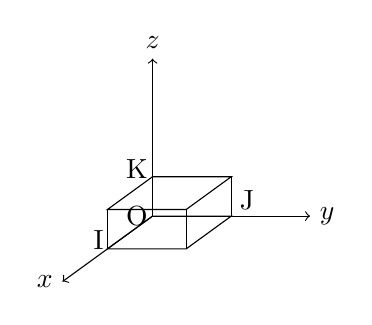
\begin{tikzpicture}[x={(-0.572cm,-0.416cm)},y={(1cm,0cm)},z={(0cm,1cm)}]
\draw[->] (0,0,0)--(2,0,0) node[left] {$x$};
\draw[->] (0,0,0)--(0,2,0) node[right] {$y$};
\draw[->] (0,0,0)--(0,0,2) node[above] {$z$};
\draw (0,0,0)--(1,0,0)--(1,1,0)--(0,1,0)--cycle;
\draw (0,0,0.5)--(1,0,0.5)--(1,1,0.5)--(0,1,0.5)--cycle;
\draw (0,0,0)--(0,0,0.5);
\draw (1,0,0)--(1,0,0.5);
\draw (0,1,0)--(0,1,0.5);
\draw (1,1,0)--(1,1,0.5);
\node  at (1.2,0,0.2) {I};
\node  at (0,1.2,0.2) {J};
\node  at (0,-0.2,0.6) {K};
\node  at (0,-0.2,0) {O};

\end{tikzpicture}

 \begin{theorem}[admis]
 Le volume de la partie d'un solide limité par les plan $ \mathcal{P}_{a} $ et $ \mathcal{P}_{b} $ d'équation respective $z = a$ et $z = b$  en unité de volume est :
 \[V= \inte{a}{b}{S(t)}{t}   \]
Où $ S(t) $ est l'aire de la section du solide par le plan
d'équation $z = t$, avec S continue sur $ \intff{a}{b} $
 \end{theorem}

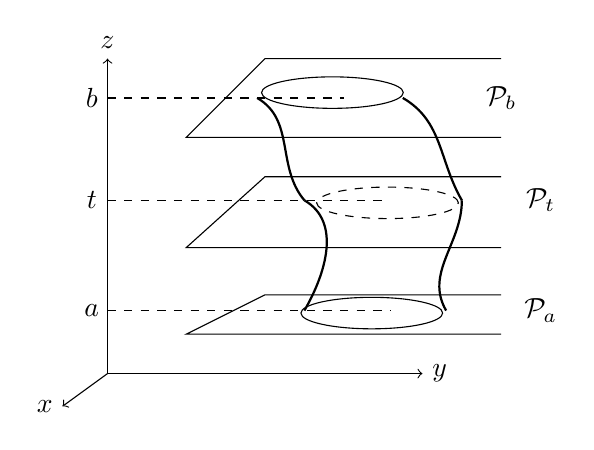
\begin{tikzpicture}[x={(-0.572cm,-0.416cm)},y={(1cm,0cm)},z={(0cm,1cm)}]
\draw[->] (0,0,0)--(1,0,0) node[left] {$x$};
\draw[->] (0,0,0)--(0,4,0) node[right] {$y$};
\draw[->] (0,0,0)--(0,0,4) node[above] {$z$};
\draw (0,5,0.5)--(0,1,0.5)--(0,2,1)--(0,5,1);
\node  at(0,-0.2, 3.5) {$ b $};
\draw[dashed] (0,0,3.5,) -- (0,3,3.5);
\node  at(0,-0.2, 2.2) {$ t $};
\draw[dashed] (0,0,2.2) -- (0 ,3.5,2.2);
\node  at(0,-0.2, 0.8) {$ a $};
\draw[dashed] (0,0,0.8) -- (0 ,3.6,0.8);
\draw (0,5,3)--(0,1,3)--(0,2,4)--(0,5,4);
\draw (0,5,1.6)--(0,1,1.6)--(0,2,2.5)--(0,5,2.5);
\draw(2,4,4.4) ellipse (0.9cm and 0.2cm);
\draw[dashed] (2,4.7,3) ellipse (0.9cm and 0.2cm);
\draw(2,4.5,1.6) ellipse (0.9cm and 0.2cm);
\draw[thick ,out=-30,in=120](0,3.75,3.5)to(0,4.5,2.2);
\draw[thick ,out=-30,in=130](0,1.9,3.5)to(0,2.5,2.2);
\draw[thick ,out=-90,in=120](0,4.5,2.2)to(0,4.3,0.8);
\draw[thick ,out=-30,in=60](0,2.5,2.2)to(0,2.5,0.8);
\node  at (0,5,3.5) {$ \mathcal{P}_{b} $};
\node  at (0,5.5,0.8) {$ \mathcal{P}_{a} $};
\node  at (0,5.5,2.2) {$ \mathcal{P}_{t} $};
\end{tikzpicture}


\subsection*{Calcul de volumes de solides de révolution}
On considère, dans un repère orthonormé, la fonction $f$ définie sur $\intff{0}{1}$ par :
\[ f(x)=\sqrt{x}+x. \]
\`A partir de sa courbe représentative (en trait épais ci-dessous), on engendre un volume en la faisant tourner autour de l'axe des abscisses, comme indiqué sur le graphique suivant :

\begin{center}
\begin{tikzpicture}[scale=3]
\draw[thick,->,>=stealth'] (0,0) -- (1.5,0);
\draw[thick,->,>=stealth'] (0,-.3) -- (0,.3);
\draw[very thick] plot[domain=0:1,samples=70] (\x,{sqrt(\x)-\x});
\draw plot[domain=0:1,samples=70] (\x,{-sqrt(\x)+\x});
\draw (0.7,{sqrt(0.7)-0.7}) arc (90:270:0.05 cm and 0.137 cm);
\draw[dotted] (0.7,{-sqrt(0.7)+0.7}) arc (-90:90:0.05 cm and 0.137 cm);
\draw[dotted] (0.7,0)--(0.7,{sqrt(0.7)-0.7});
%
\draw (0.4,{sqrt(0.4)-0.4}) arc (90:270:0.05 cm and 0.232 cm);
\draw[dotted] (0.4,{-sqrt(0.4)+0.4}) arc (-90:90:0.05 cm and 0.232 cm);
\draw[dotted] (0.4,0)--(0.4,{sqrt(0.4)-0.4});
\node[below left,scale=0.7] at (0,0) {0};
\node[below right,scale=0.7] at (1,0) {1};
\draw[<-,>=stealth'] (0.4,0.116) to[bend left=30] (0.6,0.3) node[right,scale=0.7] {disque de rayon $f(x)$};
\end{tikzpicture}
\end{center}

On peut voir ce volume comme la somme des aires des disques de rayon $f(x)$, pour $x$ variant de $0$ à $1$. Un de ces disques a pour aire : $\pi\left(f(x)\right)^2$.\\
Ainsi, le volume peut se calculer par :

$
\inte{0}{1}{\pi\left(f(x)\right)^2}{x}  = \inte{0}{1}{\pi\left(\sqrt{x}+x\right)^2}{x}\\
 = \inte{0}{1}{\pi\left(x+2x\sqrt{x}+x^2\right)}{x}\\
 = \pi \inte{0}{1}{ x}{x} + 2\pi\inte{0}{1}{x\sqrt{x}}{x} + \pi\inte{0}{1}{x^2}{x}$


Posons :
\[ I =\inte{0}{1}{x\sqrt{x}}{x} \]
et calculons-là à l'aide d'une intégration par parties.\\
On pose alors : $u(x)=\sqrt{x},\quad $ $v'(x)=x$ et donc $u'(x)=\dfrac{1}{2\sqrt{x}}$ et $v(x)=\dfrac{1}{2}x^2$. D'où :

$I  = \left[\dfrac{1}{2}x^2\sqrt{x}\right]_0^1-\inte{0}{1}{\dfrac{1}{4}\dfrac{x^2}{\sqrt{x}}}{x}\\
I = \dfrac{1}{2}-\dfrac{1}{4}\inte{0}{1}{x\sqrt{x}}{x}\\
I = \dfrac{1}{2}-\dfrac{1}{4}I$


On en déduit alors que $\dfrac{5}{4}I=\dfrac{1}{2}$, soit : $I=\dfrac{2}{5}.$\\
Le volume cherché est donc :

$\inte{0}{1}{\pi\left(f(x)\right)^2}{x}  = \pi\left[\dfrac{1}{2}x^2\right]_0^1+\dfrac{4\pi}{5}+\pi\left[\dfrac{1}{3}x^3\right]_0^1
 = \dfrac{\pi}{2}+\dfrac{4\pi}{5}+\dfrac{\pi}{3}
 = \dfrac{49\pi}{30}.$


Nous donnons  ci-dessous la formule donnant le volume du solide  de revolution engendré par la rotation d'un arc de courbe autour de l'axe (O,x).

\begin{property}
 L'espace est muni d'un repère  orthonormé $ \oijk. $\\
  Soit $f$ une fonction continue   et positive sur $[a, b]$. Le  volume  V du solide  de révolution engendré par la rotation de la courbe $ \mathcal{C}_{f}\; $    autour de l'axe $(O,\overrightarrow{i} ) $  est  le réel:\; V$ =\pi \inte{a}{b}{f^{2}(x)}{x}  $  en unité de volume.
  
 \end{property} 
 
  %</content>
\end{document}